\documentclass[10pt,letterpaper]{article}
\usepackage{tools}
\usepackage{enumitem}
%\settextfont{B Nazanin}
\usepackage{lipsum}
\setlength{\parskip}{3mm}
\setlength{\parindent}{0mm}
\newcommand{\wid}{0.49\textwidth}
\newcommand{\widone}{60mm}
\begin{document}
\Large
\begin{center}
In the name of beauty

8th problem set solution of ComNet course
\hl
\end{center}
Q1)
\begin{enumerate}[label=\alph*-]
\item
False. The only information each node distributes to its neighbors is its own DV.
\item
True. Poisoned Reverse does the trick by allowing for white lies whenever needed.
\item
True. The fact that routers become aware of the state of a network simultaneously leads to routing oscillations which is almost removed through asynchronization.
\item
False. RIP (Routing Information Protocol) is an \textbf{intra-AS} protocol and runs on top of the \textbf{DV} algorithm.
\item
True. Both are parts of BGP, which is responsible for distributing proper information to each and every bit of ASs.
\end{enumerate}
Q2) 
\begin{enumerate}[label=\alph*-]
\item
\begin{figure}[htbp]
\centering
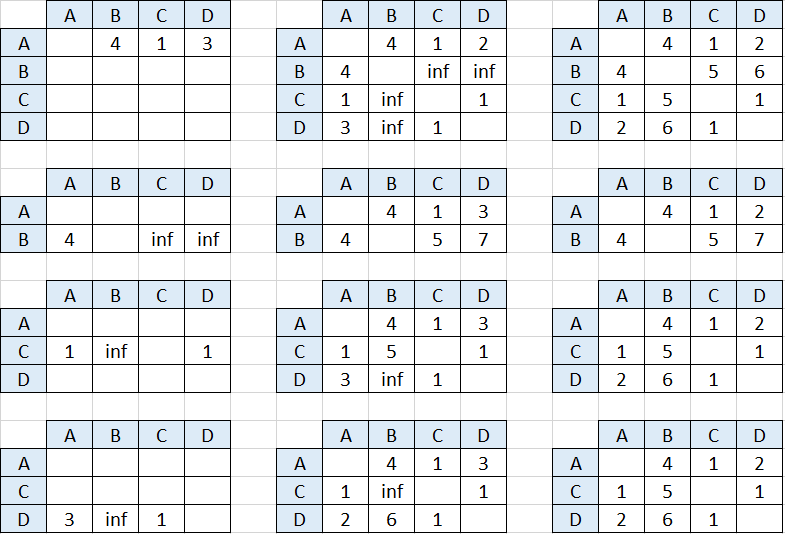
\includegraphics[width=110mm]{DV.png}
\end{figure}
\item
After the AC link cost increases to 10, node C, knowing this change, forwards all the packets destined for either node A or node B to node D. Node D forwards the packet to C since it considers this node as its predecessor on the way to node A. Another alteration is where node A wants to send packets to node C. It runs the DV algorithm locally and finds the new optimum path A-D-C.
\item
Node D advertises its distance to node A or node B as $\infty$ to node C.
\begin{figure}[htbp]
\centering
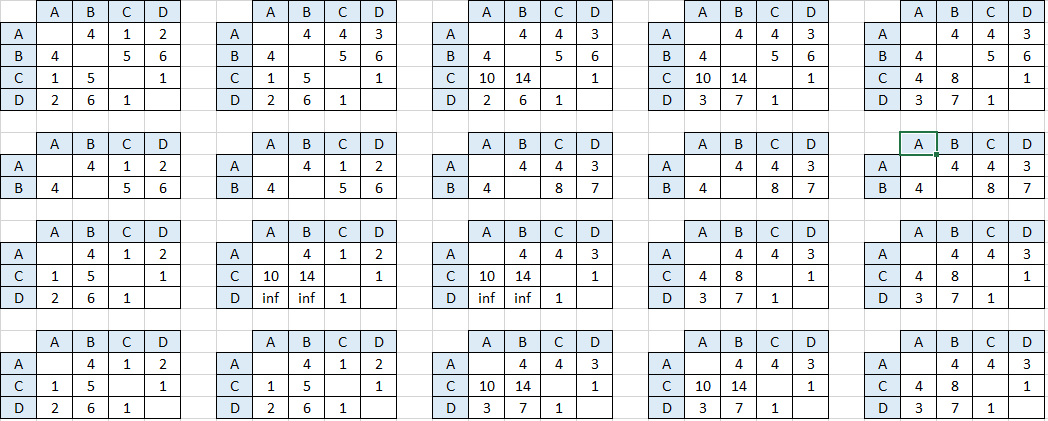
\includegraphics[width=140mm]{DV_PR.png}
\end{figure}
\end{enumerate}

Q3) 
\begin{enumerate}[label=\alph*-]
\item
In the uncontrolled flooding scheme, the total transmitted packet size is $\infty$, since all the nodes keep forwarding a specific packet forever.
\item
In this case, a packet is accepted and duplicated to all other links only if the packet has arrived on its shortest path to the source node (node A).

Node A sends two copies of the packet to nodes B and D.

Node B sends a copy of the packet to node G.

Node D sends two copies of the packet to nodes C and E.

Nodes C and E receive two copies of the packet from node D and send to each other, which are eventually dropped since they did not arrive on the shortest paths to node A.

Node E also forwards the packet to node F and the transmission is complete.

A total of $8\times 5=40$Kbytes of data is carried over the network.
\item
minimum-spanning tree with center-based approach
Assuming the center node to be node A, we have the following steps of establishing the tree:
\begin{enumerate}
\item
Node B joins to node A through direct link.
\item
Node G joins to the tree through node B.
\item
Node D joins to node A through direct link.
\item
Node C joins to the tree through node D.
\item
Node E joins to the tree through node D.
\item
Node F joins to the tree through node E.
\end{enumerate}
A total of $6\times 5=30$Kbytes of data is displaced.
\end{enumerate}
%(In part c-, also fully explain the steps of attaining such spanning tree.)
%\begin{figure}[htbp]
%\centering
%\includegraphics[width=120mm]{broadcast.pdf}
%\end{figure}

Q4) In the following network (next page), a group of nodes, denoted by red, decide to join a multicast group and all other nodes (denoted by black) are inactive for the multicast session. The source node is attached to router A.
\begin{enumerate}[label=\alph*-]
\item
A, B, C, E and H
\item
Router D has this property.
\item
Routers I, G and F, having no multicast party, send a pruning message to their upstream router.
\item
BG, GI and EF
\end{enumerate}
%\begin{figure}[htbp]
%\centering
%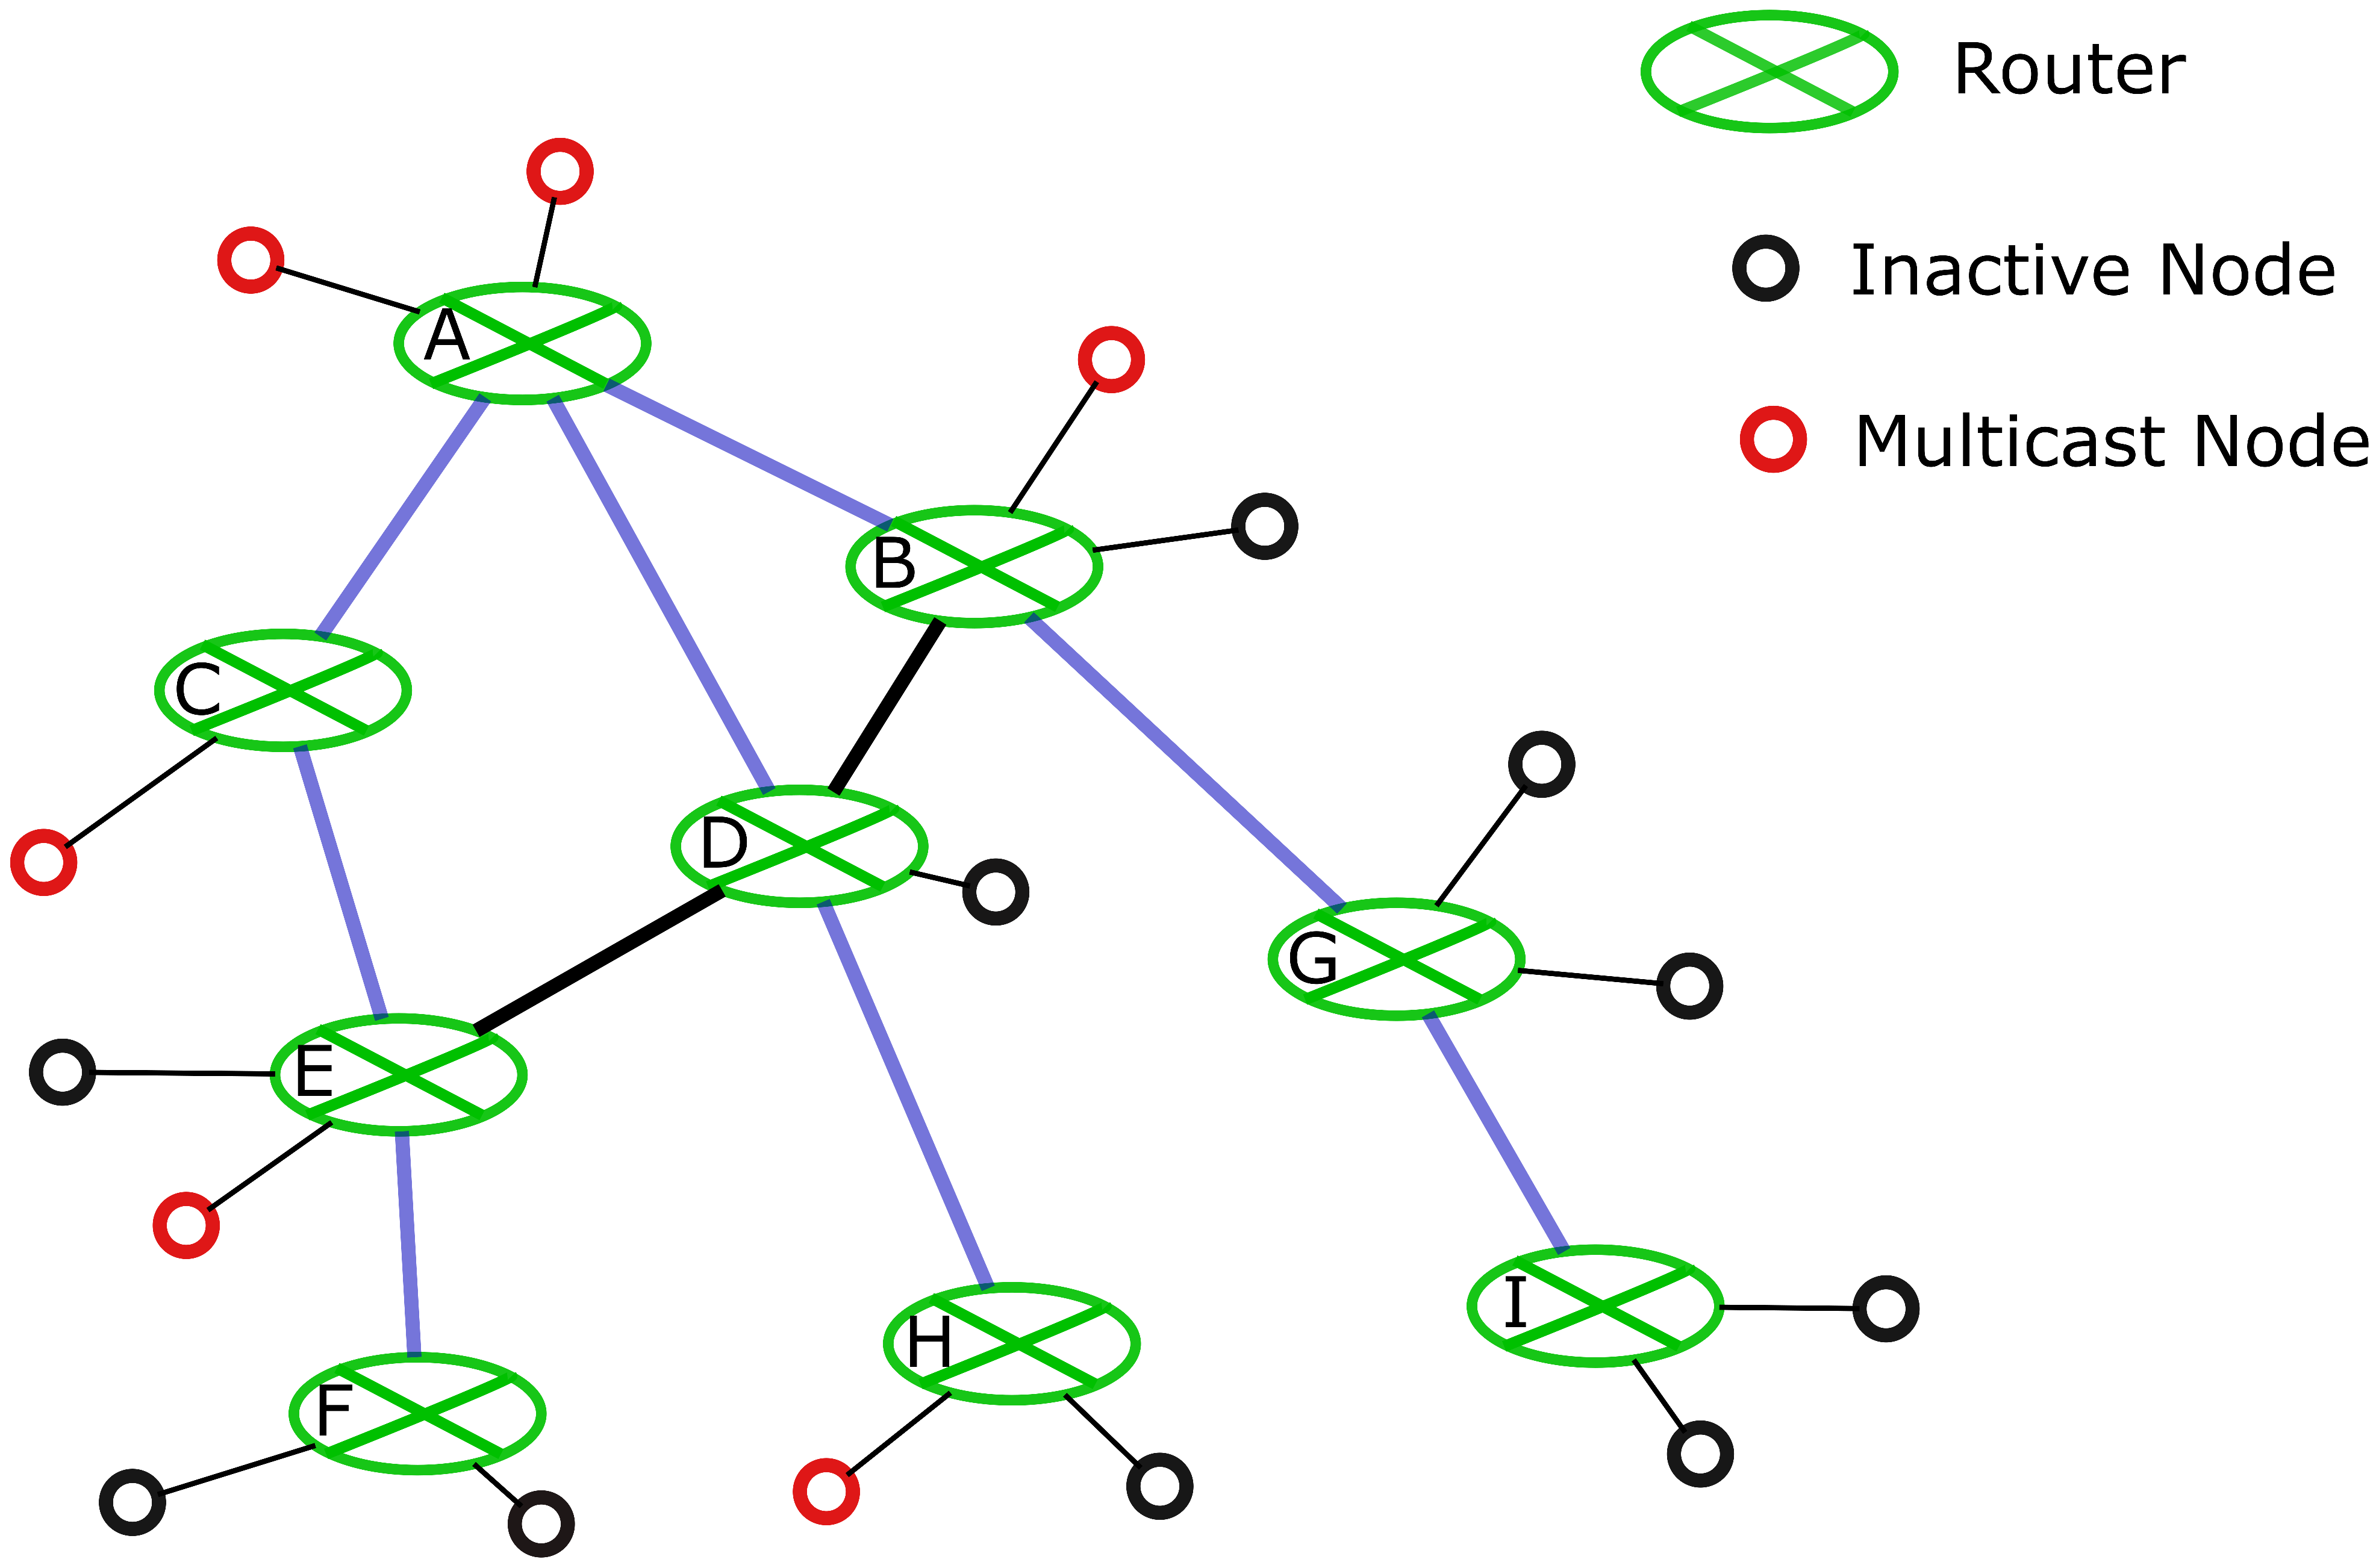
\includegraphics[width=140mm]{multicast.eps}
%\end{figure}

\end{document}